% !TeX root = RJwrapper.tex
\title{Working with figure environments in texor}
\author{by Abhishek Ulayil}

\maketitle

\abstract{
This is a small sample article to demonstrate usage of texor to convert figure environments.
}

\section{Introduction}

Images are an essential component in any article, However due to the differences in the support for various graphic formats between LaTeX and markdown/HTML we need to fallback on raster graphics. 
It is well summarized in the table \ref{table:1}

\begin{table}[htbp]
\centering
\begin{tabular}{l | llll }
 \hline
 Graphics Format & LaTeX & Markdown & Rmarkdown & HTML \\
 \hline
 PNG       & Yes & Yes & Yes & Yes \\
 JPG       & Yes & Yes & Yes & Yes \\
 PDF       & Yes & No & No & No \\
 SVG       & No & Yes & Yes & Yes \\
 Tikz      & Yes & No & Yes & No \\
 Algorithm & Yes & No & No & No \\
\hline
\end{tabular}
\caption{Image Format support in various Markup/Typesetting Languages}
\label{table:1}
\end{table}


\section{Image with width parameters}
This section may contain a figure such as Figure~\ref{figure:rlogo}.
This is the most basic example of figure.

\begin{verbatim}
\begin{figure}[htbp]
  \centering
  \includegraphics[width=0.35\textwidth]{Rlogo-5.png}
  \caption{The logo of R.}
  \label{figure:rlogo}
\end{figure}
\end{verbatim}

\begin{figure}[htbp]
  \centering
  \includegraphics[width=0.35\textwidth]{Rlogo-5.png}
  \caption{The logo of R.}
  \label{figure:rlogo}
\end{figure}


\section{Images in PDF format}

Image \ref{fig:normal} is a graphical representation of normal distribution.

\begin{verbatim}
\begin{figure}[htbp]
  \centering
  \includegraphics[width=0.5\textwidth]{normal}
  \caption{PDF of a normal distribution}
  \label{fig:normal}
\end{figure}
\end{verbatim}
\begin{figure}[htbp]
  \centering
  \includegraphics[width=0.5\textwidth]{normal}
  \caption{PDF of a normal distribution}
  \label{fig:normal}
\end{figure}

\section{Multiple images}
 Pandoc v3 and above now supports a new Figure object \citep{pandoc} which supports multiple 
 images side by side or in a grid format.
%% Two images side by side
\subsubsection{Two or more Images side by side}
\begin{verbatim}
\begin{figure}[htbp]
  \centering
  \includegraphics[width=0.45\textwidth]{Rlogo-5.png}\includegraphics[width=0.45\textwidth]{normal}
  \caption{Images side by side}
  \label{fig:twoimages}
\end{figure}
\end{verbatim}

\begin{figure*}[htbp]
  \centering
  \includegraphics[width=0.45\textwidth]{Rlogo-5.png}\includegraphics[width=0.45\textwidth]{normal}
  \caption{Images side by side}
  \label{fig:twoimages}
\end{figure*}

%% Four images in a grid
\subsubsection{Four Images in a grid}

\begin{verbatim}
\begin{figure}[htbp]
  \centering
  \includegraphics[width=0.45\textwidth]{Rlogo-5.png}\includegraphics[width=0.45\textwidth]{normal}
  \includegraphics[width=0.45\textwidth]{normal}\includegraphics[width=0.45\textwidth]{Rlogo-5.png}
  \caption{Multiple images in a grid}
  \label{fig:fourimages}
\end{figure}

\end{verbatim}

\begin{figure}[htbp]
  \centering
  \includegraphics[width=0.45\textwidth]{Rlogo-5.png}\includegraphics[width=0.45\textwidth]{normal}
  \includegraphics[width=0.45\textwidth]{normal}\includegraphics[width=0.45\textwidth]{Rlogo-5.png}
  \caption{Multiple images in a grid}
  \label{fig:fourimages}
\end{figure}


\section{Tikz images}

Here is a tikz image example in fig \ref{fig:tikz} adapted from \citep{casflow}.


Another interesting aspect of including tikz image here is that you can modify the
source and re-convert without making any other changes. Figure will get updated
in the generated html article.

\subsubsection{Tikz Code:}
\begin{verbatim}
\begin{figure}

%% Generated Image will included as a PNG above automatically
  \centering
\tikzstyle{process} = [rectangle, rounded corners,
minimum width=3cm, 
minimum height=1cm,
text centered, 
draw=black]
\tikzstyle{arrow} = [thick,->,>=stealth]
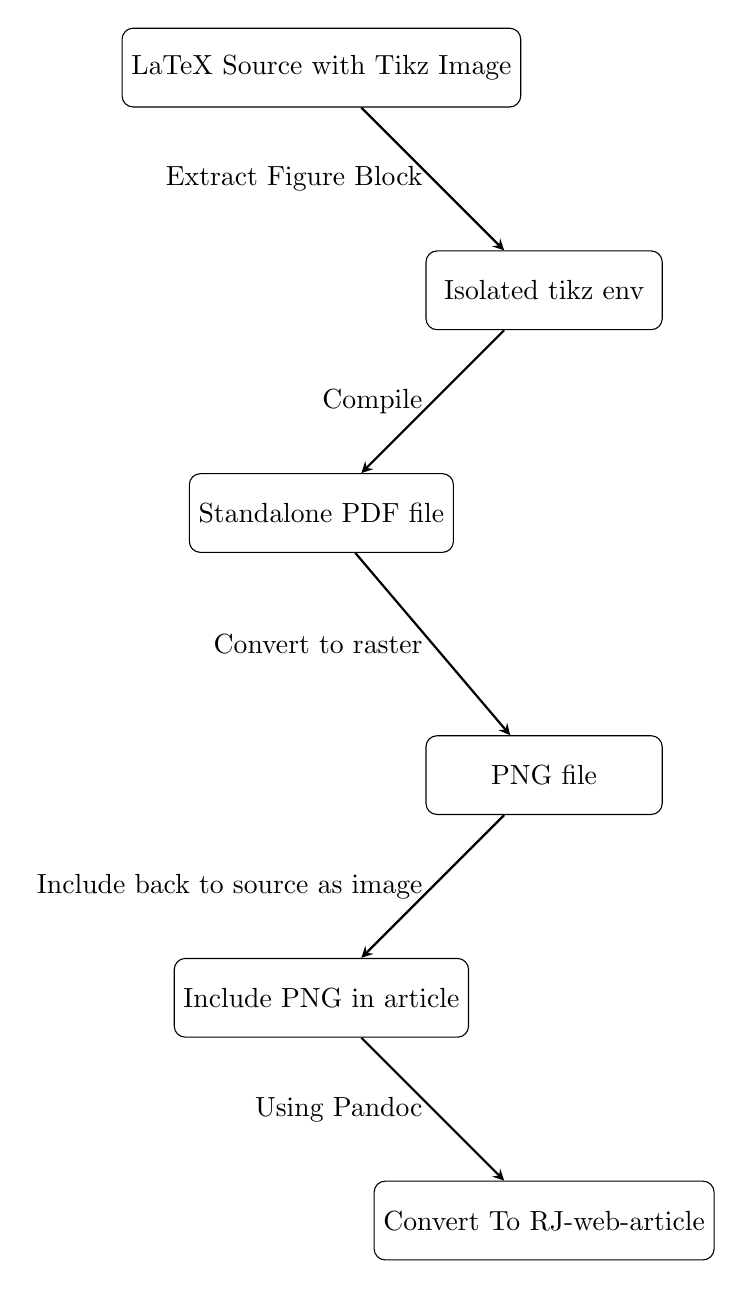
\begin{tikzpicture}[node distance=4cm]
%Nodes
\node (start) [process] {LaTeX Source with Tikz Image};
\node (isolate) [process, below right of=start] {Isolated tikz env};
\node (pro1) [process, below left of=isolate] {Standalone PDF file};
\node (pro2) [process, below right of=pro1, yshift=-0.5cm] {PNG file};
\node (link) [process, below left of=pro2] {Include PNG in article};
\node (stop) [process, below right of=link] {Convert To RJ-web-article};
% arrows
\draw [arrow] (start) -- node[anchor=east] {Extract Figure Block} (isolate);
\draw [arrow] (isolate) -- node[anchor=east] {Compile} (pro1);
\draw [arrow] (pro1) -- node[anchor=east] {Convert to raster} (pro2);
\draw [arrow] (pro2) -- node[anchor=east] {Include back to source as image} (link);
\draw [arrow] (link) -- node[anchor=east] {Using Pandoc} (stop);
\end{tikzpicture}
\caption{Tikz Image example}
  \label{fig:tikz}
\end{figure}

\end{verbatim}

\subsubsection{Resultant Figure :}
\begin{figure*}

%% Generated Image will included as a PNG above
  \centering
\tikzstyle{process} = [rectangle, rounded corners,
minimum width=3cm, 
minimum height=1cm,
text centered, 
draw=black]
\tikzstyle{arrow} = [thick,->,>=stealth]
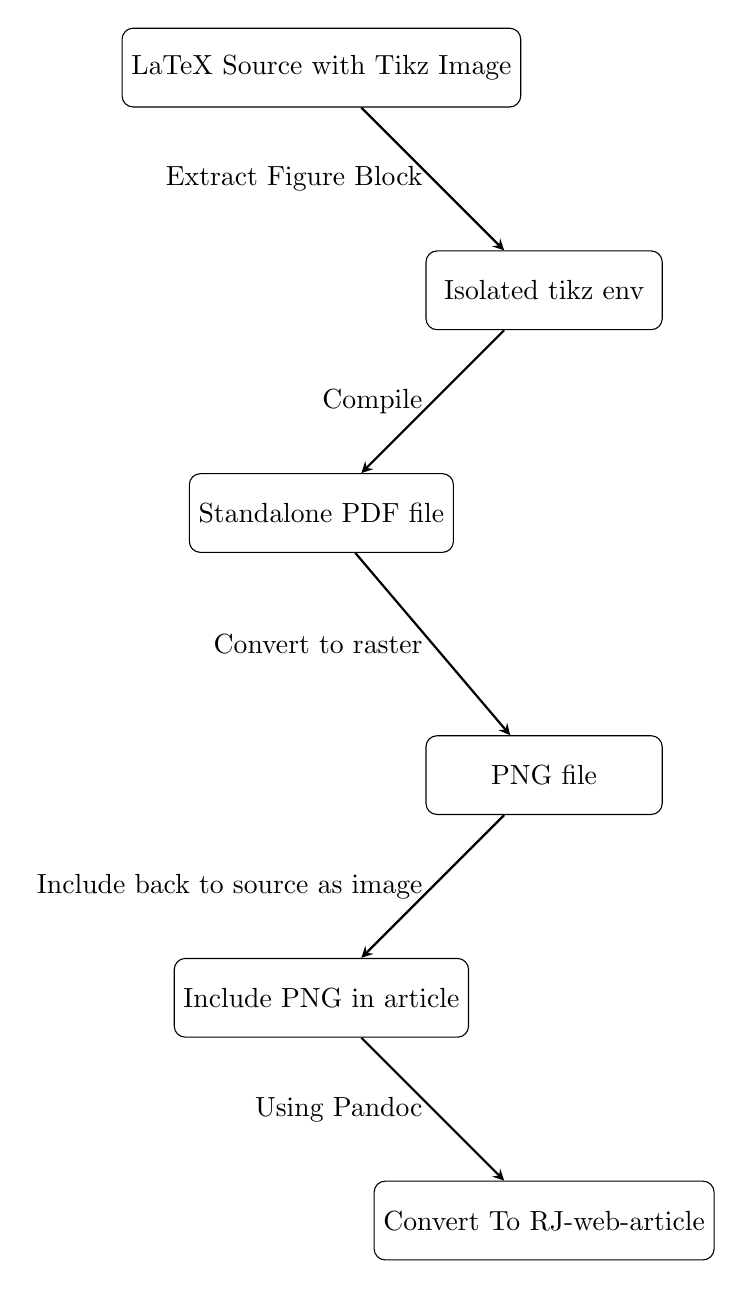
\begin{tikzpicture}[node distance=4cm]
%Nodes
\node (start) [process] {LaTeX Source with Tikz Image};
\node (isolate) [process, below right of=start] {Isolated tikz env};
\node (pro1) [process, below left of=isolate] {Standalone PDF file};
\node (pro2) [process, below right of=pro1, yshift=-0.5cm] {PNG file};
\node (link) [process, below left of=pro2] {Include PNG in article};
\node (stop) [process, below right of=link] {Convert To RJ-web-article};
% arrows
\draw [arrow] (start) -- node[anchor=east] {Extract Figure Block} (isolate);
\draw [arrow] (isolate) -- node[anchor=east] {Compile} (pro1);
\draw [arrow] (pro1) -- node[anchor=east] {Convert to raster} (pro2);
\draw [arrow] (pro2) -- node[anchor=east] {Include back to source as image} (link);
\draw [arrow] (link) -- node[anchor=east] {Using Pandoc} (stop);
\end{tikzpicture}
\caption{Tikz Image example}
  \label{fig:tikz}
\end{figure*}


\section{Algorithm2e diagrams}

we do support algorithm2e diagrams and images, these will be numbered differently
and we strongly suggest to use "alg:" in labels for best results. 
Here is an example of algorithm \ref{alg:how}, referenced from \cite{algoexample}

\begin{verbatim}
\begin{algorithm}[htbp]
\SetAlgoLined
\KwData{this text}
\KwResult{how to write algorithm with \LaTeX2e }
initialization\;
\While{not at end of this document}{
read current\;
\eIf{understand}{
go to next section\;
current section becomes this one\;
}{
go back to the beginning of current section\;
}
}
\caption{How to write algorithms}
  \label{alg:how}
\end{algorithm}
\end{verbatim}

\begin{algorithm}[htbp]
\SetAlgoLined
\KwData{this text}
\KwResult{how to write algorithm with \LaTeX2e }
initialization\;
\While{not at end of this document}{
read current\;
\eIf{understand}{
go to next section\;
current section becomes this one\;
}{
go back to the beginning of current section\;
}
}
\caption{How to write algorithms}
  \label{alg:how}
\end{algorithm}

\section{Other elements in figure objects}
Figures can also house non-image environments like CodeBlocks and Para. This 
also creates an opportunity to add support for CodeBlock numbering with some
lua filter trickery.
\begin{figure}[htbp]
\begin{center}
\begin{verbatim}
code_in_figure <- function() {
  if (pandoc_version >= 3) {
    print("Code in Figure Supported")
  }
  else {
    print("code in Figure not supported")
  }
}
\end{verbatim}
\caption{ Example Code inside Figure environment}
\label{code:example}
\end{center}
\end{figure}
\section{Summary}

In summary the \CRANpkg{texor} package supports:
\begin{itemize}
\item Almost all image formats in LaTeX.
\item Algorithm and tikz as well in some capacity.
\item Multiple images in grid,side-by-side configuration.
\item Image Captions with Numbering and Labelling.
\end{itemize}



\begin{thebibliography}{4}
    \providecommand{\natexlab}[1]{#1}
    \providecommand{\url}[1]{\texttt{#1}}
    \expandafter\ifx\csname urlstyle\endcsname\relax
      \providecommand{\doi}[1]{doi: #1}\else
      \providecommand{\doi}{doi: \begingroup \urlstyle{rm}\Url}\fi
\bibitem[Cassidy(2013)]{casflow}
Josh Cassidy
\newblock LaTeX Graphics using TikZ: A Tutorial for Beginners (Part 3)—Creating Flowcharts
\newblock \emph{Overleaf tutorials} \penalty0 2013
\newblock URL \url{https://www.overleaf.com/learn/latex/}

\bibitem[Fiorio (2017)]{algoexample}
Christophe Fiorio
\newblock algorithm2e.sty — package for algorithms, release 5.2
\newblock \emph{CTAN},\penalty0 2017
\newblock URL \url{https://mirror.kku.ac.th/CTAN/macros/latex/contrib/algorithm2e/doc/algorithm2e.pdf}

\bibitem[Krewinkel, Lucero (2023)]{pandoc}
Albert Krewinkel and Aner Lucero
\newblock pandoc 3.0 Release notes
\newblock \emph{pandoc} \penalty0 2023
\newblock URL \url{https://pandoc.org/releases.html#pandoc-3.0-2023-01-18}

\end{thebibliography}


\address{%
Abhishek Ulayil\\
Student, Institute of Actuaries of India\\%
Mumbai, India\\
ORCiD: 0009-0000-6935-8690\\
}
